
\begin{figure}\centering
    \begin{tabular}{@{}c@{\hspace{1mm}}c@{\hspace{4mm}}c@{\hspace{1mm}}c@{}}
        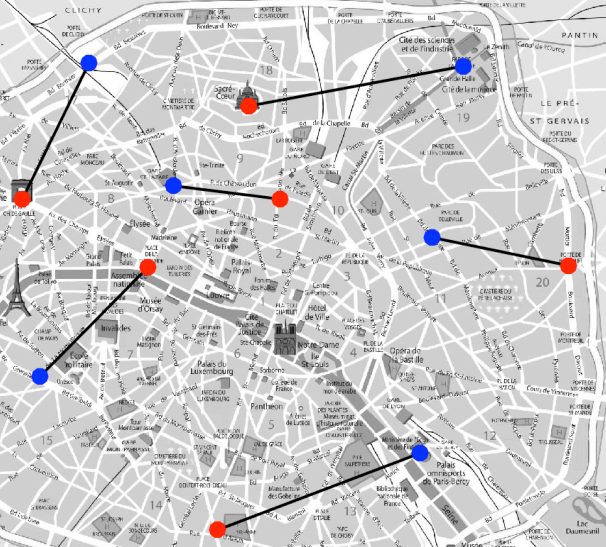
\includegraphics[width=.22\linewidth]{transport/cafe-paris/ordre-croissant-64}&
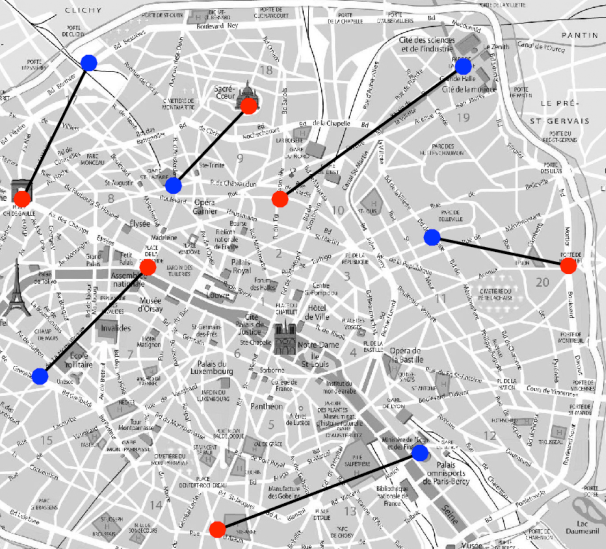
\includegraphics[width=.22\linewidth]{transport/cafe-paris/ordre-croissant-65}&
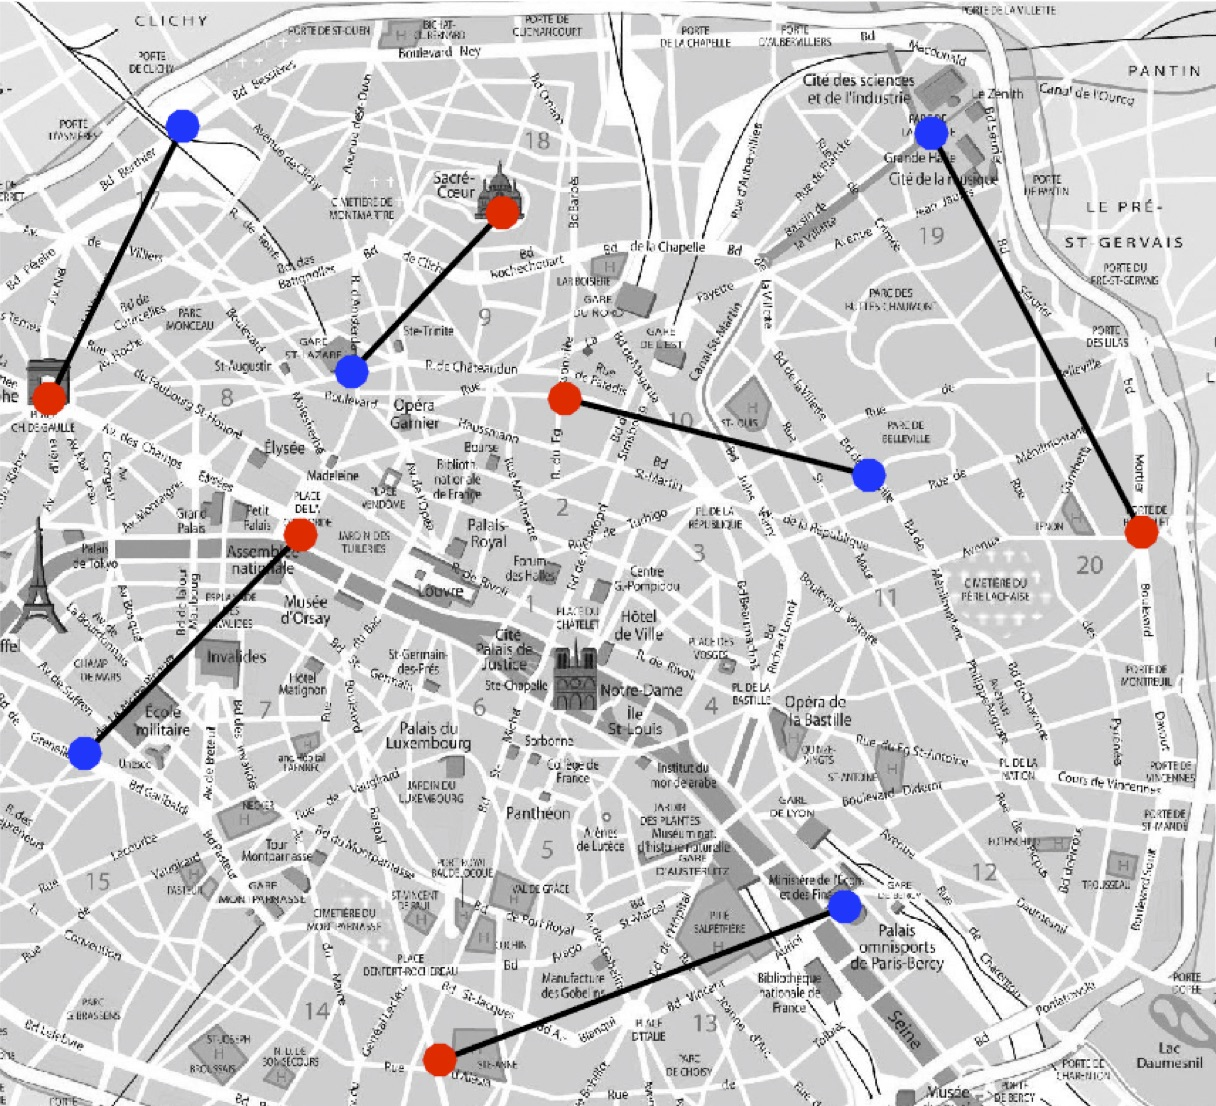
\includegraphics[width=.22\linewidth]{transport/cafe-paris/ordre-croissant-66}&
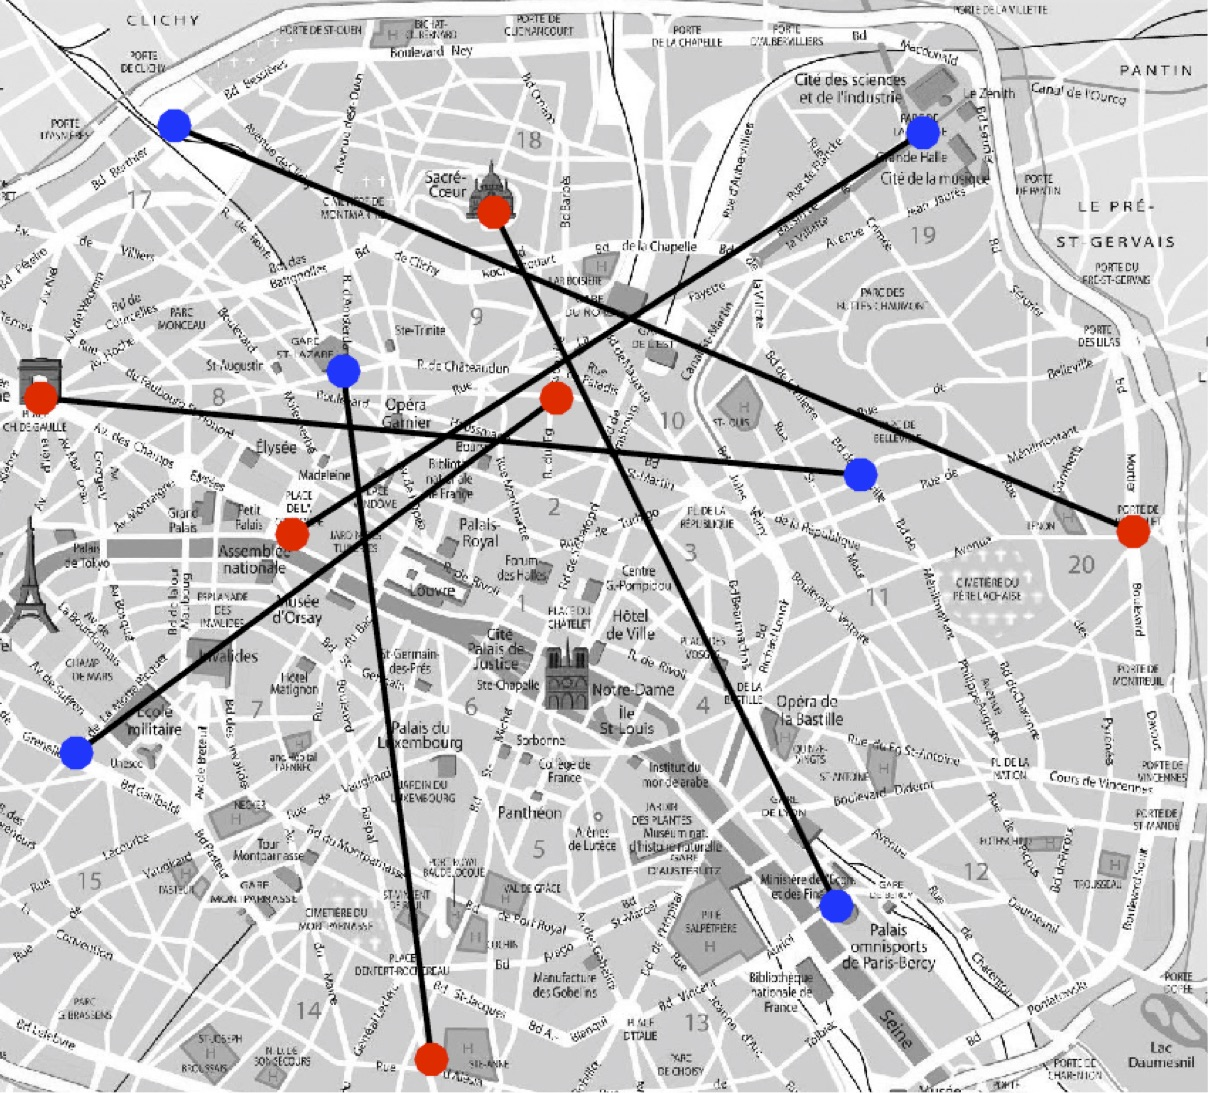
\includegraphics[width=.22\linewidth]{transport/cafe-paris/ordre-croissant-152}\\
Coût=64 &  
Coût=65 &  
Coût=66 &  
Coût=152
    \end{tabular}
    \caption{\label{fig:ordre-croissant} Matrice de coût et connexions associées. Gauche: une ligne de la matrice coût. Droite: un choix de permutation valide. } 
\end{figure}

 
